\section{System Architecture}
\label{sec:architecture}

Mine Memristors is built on Fabric, a lightweight, widely used modding toolchain for
Minecraft. The codebase is organized into five packages, shown in
Figure~\ref{fig:architecture}: a solver package with no dependency on any Minecraft class at
all, a pair of packages describing the in-world blocks and their per-block simulation
state, a networking/topology package that ties placed blocks together into a circuit and
synchronizes probe readings to clients, and a client-only package responsible for rendering
the oscilloscope heads-up display.

\begin{figure}[htbp]
\centering
\begin{tikzpicture}[
    box/.style={draw, rounded corners, minimum width=6.2cm, minimum height=1cm,
                align=center, font=\small},
    node distance=0.45cm
]
\node[box, fill=gray!10] (sim) {\texttt{sim} --- pure-Java MNA circuit solver\\(no Minecraft dependency)};
\node[box, below=of sim, fill=blue!8] (blockentity) {\texttt{blockentity} --- per-block simulation state\\(components, wire/ground nodes, modules)};
\node[box, below=of blockentity, fill=blue!8] (block) {\texttt{block} --- placement, orientation, right-click interaction};
\node[box, below=of block, fill=orange!12] (network) {\texttt{network} --- topology construction, solve loop,\\multi-channel probe protocol};
\node[box, below=of network, fill=green!10] (client) {\texttt{client} --- oscilloscope HUD rendering (client-side only)};

\draw[-{Latex[length=2mm]}] (blockentity) -- (sim);
\draw[-{Latex[length=2mm]}] (block) -- (blockentity);
\draw[-{Latex[length=2mm]}] (network) -- (blockentity);
\draw[-{Latex[length=2mm]}] (network) -- (sim);
\draw[-{Latex[length=2mm]}] (client) -- (network);
\end{tikzpicture}
\caption{Package-level architecture. The solver has zero Minecraft dependencies and is
directly unit-testable with plain \texttt{javac}/\texttt{java}; every other layer builds on
it.}
\label{fig:architecture}
\end{figure}

\subsection{Components and topology}

Every two-terminal component (resistor, capacitor, inductor, memristor, the two voltage
sources, and an ammeter) occupies a single block, oriented along the horizontal or vertical
axis the player was facing when it was placed; its two electrical leads are its front and
back faces along that axis, and its other four faces are electrically insulated. A separate
wire block conducts on all six faces and has no orientation, and a ground block (see
Section~\ref{sec:circuit-solver}) behaves identically to wire for topology purposes.

Once per game tick, for each independent group of adjacent, mutually-conductive blocks
(a ``network''), the mod rebuilds a union--find partition over every block face that
presents a conductive surface toward a conductive neighbor, assigns one MNA node index to
each resulting partition, and asks every component in that network to stamp itself into the
circuit between its resolved node indices. Figure~\ref{fig:gallery} shows the full set of
component and utility blocks available to a player.

\begin{figure}[htbp]
\centering
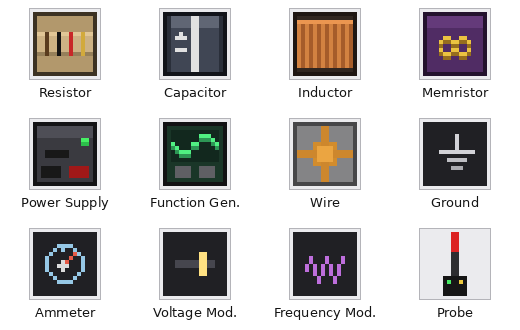
\includegraphics[width=0.85\textwidth]{figures/component_gallery.png}
\caption{The complete set of blocks and items provided by the mod.}
\label{fig:gallery}
\end{figure}

\subsection{A topology bug worth describing}
\label{sec:topology-bug}

An earlier version of the topology-construction algorithm keyed every participant in the
union--find structure by its block position alone, and unioned a component's own position
with each conductive neighbor in turn. For a plain wire block, conductive on all six faces
uniformly, this is correct: the block genuinely is a single electrical point, and merging it
with every conductive neighbor is exactly the desired behavior. For a two-terminal
component, however, this is wrong: unioning the component's position with its front
neighbor, and separately with its back neighbor, makes those two neighbors transitively
equivalent to one another \emph{through the component's own body}, because union--find
partitions are transitive. In other words, any component that had conducting material on
both of its leads simultaneously -- which is to say, any component actually wired into a
non-trivial circuit -- was silently short-circuited by the very algorithm meant to wire it
in, regardless of orientation or which component type it was. The fix, verified by
replaying a real in-world circuit's saved block data through both versions of the
algorithm offline, is to give a two-terminal component two independent partition
identities, one per lead, keyed by (position, side) rather than by the bare block position,
so that its two terminals can only be unified with one another by an actual external
connection, never by the component's own presence in the graph. Wire and ground blocks,
which are genuinely single electrical points, keep the simpler bare-position identity. This
episode is included here because it is a useful illustration for students in its own right:
a circuit topology bug that produces a mathematically singular system (a voltage source or
resistor with both terminals forced to the same node) is a natural, concrete example of why
a solver needs defensive numerical handling (Section~\ref{sec:circuit-solver}) even when the
graph-construction logic that feeds it is believed correct.

\subsection{Multi-channel oscilloscope protocol}

A handheld probe item lets a player pin up to three components, wires, or ground blocks at
once (right-click to pin or promote to most-recently-used, shift-right-click to unpin); the
server streams each pinned position's instantaneous voltage, current, a 200-sample rolling
history, and a short human-readable summary to that player once per tick, and the client
renders each of the up to three channels as an independently color-coded, auto-scaled
oscilloscope trace stacked in a corner of the screen. A component's trace shows the voltage
drop across its two leads (or, for the ammeter, the branch current, reusing the same
history/rendering machinery so that current and voltage can be watched side by side with no
separate ``current channel'' concept); a wire or ground block's trace shows its single
node's absolute voltage relative to whatever ground reference the network has, discussed
next.
